\chapter{Localizaci\'on del Punto de Contacto} \label{cap_7}

La localizaci\'on del punto de contacto en problemas de transferencia de calor\index{Calor}\index{Transferencia!de calor} en materiales multicapa
o con interfaz s\'olido-s\'olido tiene diferentes aplicaciones en el campo de la ingenier\'ia. 
Puede ser aplicado en la ingenier\'ia qu\'imica, para la determinaci\'on de impurezas en diferentes materiales \cite{Aziz10,Luke53} y para 
la separaci\'on de metales por medio de pol\'imeros \cite{Rao04,Zhai18}. En 
la ingenier\'ia farmac\'eutica, para la identificaci\'on de impurezas en medicamentos \cite{Gorog00} y en la industria cosm\'etica \cite{Andrisano95}, entre muchas otras aplicaciones que exceden el alcance de esta tesis.

En este cap\'itulo se presenta un problema inverso relacionado con el problema directo que se estudi\'o en el Cap\'itulo \ref{cap_6}. 
Se propone la estimaci\'on de un nuevo par\'ametro\index{Par\'ametro}\index{Estimaci\'on!de par\'ametros} 
relacionado directamente con el problema de interfaz, \'este es la determinaci\'on del punto de contacto entre los materiales $A$ y $B$ \cite{Umbricht20b}. 

Dado que la longitud $l$ $\textbf{[m]}$ permanece constante en todo el proceso de transferencia de calor\index{Calor}\index{Transferencia!de calor}, se utiliza para la estimaci\'on\index{Estimaci\'on}, el problema en r\'egimen estacionario\index{Estado!estacionario} y \'esta se realiza a partir de
una \'unica medici\'on 
ruidosa\index{Ruido} de flujo t\'ermico\index{Flujo!t\'ermico} en el borde derecho de la barra $(x=L)$. 

Se obtiene una expresi\'on anal\'itica para la aproximaci\'on de la ubicaci\'on del punto de contacto de los materiales. Se halla una cota para el error\index{Error!de aproximaci\'on} cometido en la aproximaci\'on que depende del ruido 
en la medici\'on\index{Ruido!en la medici\'on}. Adem\'as, con la finalidad de conocer la dependencia local del par\'ametro estimado con el dato, se realiza un estudio de elasticidad\index{Elasticidad}. Ejemplos num\'ericos, de diferentes caracter\'isticas, muestran
la utilizaci\'on del m\'etodo\index{M\'etodo} propuesto.  

%%%%%% PRESENTACION DEL PROBLEMA %%%%%%%%%%%%%%%%%%%%%%%%%%%%%%%%

\section{Presentaci\'on del Problema} \label{sec:Pres_Problema7}

En esta secci\'on se presenta formalmente el problema inverso que se va a estudiar. Se busca determinar la ubicaci\'on del punto de contacto 
$(l)$ entre los materiales $A$ y $B$ bajo las hip\'otesis del Teorema \ref{teorema_Sol_Problema_Directo2_Est}.

La estimaci\'on\index{Estimaci\'on} se realiza mediante una medici\'on ruidosa\index{Ruido!en la medici\'on} de flujo\index{Flujo!t\'ermico} $q$ en $X=L$ (borde derecho de la barra). Dado que el problema est\'a en r\'egimen estacionario, el flujo es constante en toda la barra. Se denota por $q$ $\textbf{[W/m{$^{2}$}]}$ al flujo t\'ermico\index{Flujo!t\'ermico} en $x=L$ que satisface 
%
\begin{equation}
\label{Ec_Ruido_en_el_flujo}
\left |q-q_\epsilon \right | \leq \epsilon, \qquad  \epsilon >0 , \\
\end{equation}
%
donde $q_\epsilon$ representa la medici\'on del flujo\index{Flujo!t\'ermico} y $\epsilon$ el nivel de ruido\index{Ruido!en los datos} en el dato del flujo\index{Flujo!t\'ermico}. \'Este, se determina en la pr\'actica, teniendo en cuenta el error de los instrumentos\index{Error!de instrumentaci\'on} de medici\'on utilizados. 


\section{Determinaci\'on del Par\'ametro} \label{sec:Aprox_l}

En esta secci\'on se resuelve de manera anal\'itica el problema inverso de determinaci\'on en cuesti\'on, considerando que el problema de transferencia de calor\index{Calor}\index{Transferencia!de calor} se encuentra en r\'egimen estacionario\index{Estado!estacionario}. 

El siguiente resultado brinda una expresi\'on anal\'itica para el problema de estimaci\'on de $l$ que depende de los par\'ametros del modelo\index{Modelo}
y del flujo t\'ermico\index{Flujo!t\'ermico} $q$ en el borde derecho de la barra $(x=L)$.

\begin{theorem} \label{teorema_Sol_Aprox_l}
Sean $\kappa_A, \kappa_B, T_a, F, L,h,q \in \R^+$ tal que $F>T_a$, $0<l<L$, $\kappa_A \neq \kappa_B$ y
%
\begin{equation}
\label{cond_q}
q_m=\dfrac{\kappa_m \, h (F-T_a)}{Lh+\kappa_m}<q<\dfrac{\kappa_M \, h (F-T_a)}{Lh+\kappa_M}=q_M,
\end{equation}
%
donde
%
\begin{equation}
\label{cond_K_m_K_M}
\begin{cases}
\kappa_m=\min\left\{\kappa_A,\kappa_B\right\}, \\
\kappa_M=\max\left\{\kappa_A,\kappa_B\right\}.
\end{cases}
\end{equation}
%
Dada la funci\'on\index{Funci\'on} $u_e$ que satisface $u_e(\cdot) \in C^{2}\left((0,l)\right)$ y $u_e(\cdot) \in C^{2}\left((l,L)\right)$, el problema de determinaci\'on de $l$ en
%
\begin{equation}
\label{Ec_Problema_Estimacion_l}
\begin{cases} 
u''_{e}(x)=0, \qquad & 0<x<l, \\
u''_{e}(x)=0, \qquad & l<x<L, \\
u_{e}(x)=F, \qquad & x=0, \\
\kappa_B\,  u'_{e}(x)=-h\,(u_{e}(x)-T_a) , \qquad & x=L , \\
u_{e}(x^+)=u_{e}(x^-), \qquad & x=l , \\
\kappa_B \, u'_{e}(x^+)=\kappa_A \, u'_{e}(x^-), \qquad & x=l , \\
q=-\kappa_B \, u'_{e}(x) , \qquad & x=L,
\end{cases}
\end{equation}
%
tiene como soluci\'on\index{Soluci\'on}  
%
\begin{equation}
\label{Sol_l}
l=\dfrac{\kappa_A \, \kappa_B}{\kappa_B-\kappa_A}\left(\dfrac{F-T_a}{q}-\dfrac{1}{h}-\dfrac{L}{\kappa_B}\right).
\end{equation}
%        
\end{theorem}
%
\begin{proof}{Demostraci\'on:}
%
Se considera el sistema\index{Sistema} \eqref{Ec_Problema_Estimacion_l} sin la condici\'on de flujo\index{Flujo}\index{Condici\'on!de flujo} (\'ultima condici\'on). Debido al Teorema \ref{teorema_Sol_Problema_Directo2_Est} 
se conoce una relaci\'on entre la funci\'on\index{Funci\'on} $u_e$ y los par\'ametros\index{Par\'ametro} del modelo\index{Modelo} que viene dada por la expresi\'on \eqref{Sol_prob2}-\eqref{Eta_Denominador}, \'esta es
%
\begin{equation}
\label{Sol_prob3}
u_{e}(x)=
\begin{cases} 
F+\dfrac{\kappa_B \, h (T_a-F)}{\eta} x,  \qquad & 0 \leq x \leq l, \\
F+ \dfrac{l h \, (\kappa_B-\kappa_A) (T_a-F)  }{\eta}+\dfrac{\kappa_A  \, h (T_a-F)}{\eta} x,  \qquad & l<x \leq L, \\
\end{cases}
\end{equation}
%        
donde 
%
\begin{equation}
\label{Eta}
\eta=\kappa_A \, \kappa_B +\kappa_A  \, hL+(\kappa_B -\kappa_A)hl.
\end{equation}
% 
Se utiliza la condici\'on de flujo\index{Flujo}\index{Condici\'on!de flujo} del sistema\index{Sistema} \eqref{Ec_Problema_Estimacion_l} aplicada a la Ecuaci\'on\index{Ecuaci\'on} \eqref{Sol_prob3}-\eqref{Eta} y se obtiene
%
\begin{equation}
\label{Flujo}
q=-\kappa_B \, u'_{e}(L)=\dfrac{\kappa_A \,\kappa_B \,h(F-T_a)}{\eta}=\dfrac{\kappa_A \,\kappa_B \,h(F-T_a)}{\kappa_A \kappa_B +\kappa_A hL+(\kappa_B -\kappa_A)hl}.
\end{equation}
%
Se despeja $l$ de la Ecuaci\'on\index{Ecuaci\'on} \eqref{Flujo} y se obtiene la expresi\'on \eqref{Sol_l} tal como se quer\'ia demostrar.

Dado que $l$ es una funci\'on\index{Funci\'on} de $q$, corresponde ver que $q$ satisface la condici\'on necesaria y suficiente\index{Condici\'on!necesaria y suficiente} para la existencia de $l$ dada por \eqref{cond_q}-\eqref{cond_K_m_K_M}.
El problema de determinaci\'on de $l$ tiene sentido sii
%
\begin{equation*}
\label{cotas_l}
0<l<L,
\end{equation*}
%
equivalentemente
%
\begin{equation}
\label{cotas_l2}
0<\dfrac{\kappa_A \, \kappa_B}{\kappa_B-\kappa_A}\left(\dfrac{F-T_a}{q}-\dfrac{1}{h}-\dfrac{L}{\kappa_B}\right)<L.
\end{equation}
%
Ahora se analizan dos casos:

\textbf{Caso 1}:  $(\kappa_A < \kappa_B)$
Se opera algebraicamente a partir de \eqref{cotas_l2} y se obtiene
%
\begin{equation}
\label{cond_q_1}
\dfrac{\kappa_A \, h (F-T_a)}{Lh+\kappa_A}<q<\dfrac{\kappa_B \, h (F-T_a)}{Lh+\kappa_B}.
\end{equation}
%

\textbf{Caso 2}:  $(\kappa_A > \kappa_B)$
Se opera algebraicamente a partir de \eqref{cotas_l2} y se obtiene 
%
\begin{equation}
\label{cond_q_2}
\dfrac{\kappa_B \, h (F-T_a)}{Lh+\kappa_B}<q<\dfrac{\kappa_A \, h (F-T_a)}{Lh+\kappa_A}.
\end{equation}
%
Combinando las expresiones \eqref{cond_q_1} y \eqref{cond_q_2} se llega a \eqref{cond_q}-\eqref{cond_K_m_K_M} con lo que finaliza la prueba. 
%
\end{proof}
%
\begin{rem}
Notar que las expresiones \eqref{cond_q}-\eqref{cond_K_m_K_M} brindan una condici\'on necesaria y suficiente\index{Condici\'on!necesaria y suficiente} para el problema de determinaci\'on de $l$ bajo las hip\'otesis del Teorema \ref{teorema_Sol_Aprox_l}. 
\end{rem}
%
\section{Estimaci\'on del Error} \label{sec:Error7}
%
En esta secci\'on se obtiene una expresi\'on anal\'itica que acota el error\index{Error!de aproximaci\'on} cometido al aproximar la ubicaci\'on del punto de interfaz $(l)$ utilizando una medici\'on 
ruidosa\index{Ruido!en la medici\'on} de flujo t\'ermico\index{Flujo!t\'ermico} $q_\epsilon$.

Independientemente de que el flujo medido\index{Flujo!medido} $(q_\epsilon)$ cumpla las condiciones necesarias y suficientes\index{Condici\'on!necesaria y suficiente} dadas por las Ecuaciones\index{Ecuaci\'on} \eqref{cond_q}-\eqref{cond_K_m_K_M},
existir\'a un error en la estimaci\'on\index{Estimaci\'on}\index{Error!de estimaci\'on}
del punto de contacto que depender\'a directamente del error $(\epsilon)$ en la medici\'on\index{Error!de medici\'on} de flujo\index{Flujo}. 
El siguiente resultado muestra una cota para el error de estimaci\'on\index{Estimaci\'on}\index{Error!de estimaci\'on} del problema de inter\'es. 

\begin{theorem} \label{teorema_Error_Aprox_l}

Se considera el problema inverso de determinaci\'on de la ubicaci\'on del punto de interfaz $(l)$ dado por \eqref{Ec_Problema_Estimacion_l}.
Sea $l_\epsilon$ la soluci\'on\index{Soluci\'on!aproximada} de aproximaci\'on que depende de la medici\'on ruidosa\index{Ruido!en la medici\'on} de flujo\index{Flujo} $q_\epsilon$ en $x=L$. Se supone que el flujo\index{Flujo}
$q_\epsilon$ satisface las condiciones\index{Condici\'on} dadas por \eqref{Ec_Ruido_en_el_flujo}-\eqref{cond_K_m_K_M}. Entonces existe $K \in \R^+ $  tal que 
%
\begin{equation*}
\label{cota_l}
\left|l-l_\epsilon\right|\leq K,
\end{equation*}
%
donde $K$ viene dado por
%
\begin{equation*}
\label{cota_K}
K= \dfrac{\kappa_A \ \kappa_B }{\left|\kappa_B - \kappa_A\right| (F-T_a)} \left(\dfrac{Lh+\kappa_m}{\kappa_m \, h}\right)^2 \, \epsilon.
\end{equation*}
%
\end{theorem}
%
\begin{proof}{Demostraci\'on:}
%
Debido a la Ecuaci\'on\index{Ecuaci\'on} \eqref{Sol_l} se tiene que
%
\begin{equation}
\label{Sol_l_Aprox}
l_\epsilon=\dfrac{\kappa_A \, \kappa_B}{\kappa_B-\kappa_A}\left(\dfrac{F-T_a}{q_\epsilon}-\dfrac{1}{h}-\dfrac{L}{\kappa_B}\right).
\end{equation}
%       
Considerando las expresiones \eqref{Sol_l} y \eqref{Sol_l_Aprox} vale que 
%
\begin{equation*}
\label{l-l_aprox}
\left|l-l_\epsilon\right|=\left|\dfrac{\kappa_A \, \kappa_B}{\kappa_B-\kappa_A}\left(\dfrac{F-T_a}{q}-\dfrac{1}{h}-\dfrac{L}{\kappa_B}\right)-\dfrac{\kappa_A \, \kappa_B}{\kappa_B-\kappa_A}\left(\dfrac{F-T_a}{q_\epsilon}-\dfrac{1}{h}-\dfrac{L}{\kappa_B}\right)\right|,
\end{equation*}
%   
operando algebraicamente se obtiene
%
\begin{equation*}
\label{l-l_aprox2}
\left|l-l_\epsilon\right|=\left|\dfrac{\kappa_A \, \kappa_B}{\kappa_B-\kappa_A}\left(\dfrac{F-T_a}{q}-\dfrac{F-T_a}{q_\epsilon}\right)\right|,
\end{equation*}
% 
equivalentemente
%
\begin{equation}
\label{l-l_aprox3}
\left|l-l_\epsilon\right|=\left|\dfrac{\kappa_A \, \kappa_B}{\kappa_B-\kappa_A}\right| \dfrac{F-T_a}{q \, q_\epsilon} \left|q-q_\epsilon\right|.
\end{equation}
% 
En funci\'on\index{Funci\'on} de la condici\'on\index{Condici\'on} \eqref{cond_q}-\eqref{cond_K_m_K_M} se tiene que 
%
\begin{equation}
\label{cond_q_q_Aprox}
q, \, q_\epsilon>\dfrac{\kappa_m \, h (F-T_a)}{Lh+\kappa_m},
\end{equation}
%
utilizando la condici\'on\index{Condici\'on} \eqref{cond_q_q_Aprox} aplicada a \eqref{l-l_aprox3} vale que
%
\begin{equation*}
\left|l-l_\epsilon\right|\leq\left|\dfrac{\kappa_A \, \kappa_B}{(\kappa_B-\kappa_A) (F-T_a)}\right| \left(\dfrac{Lh+\kappa_m}{\kappa_m \, h}\right)^2 \left|q-q_\epsilon\right|,
\end{equation*}
% 
por \'ultimo, en funci\'on\index{Funci\'on} de la condici\'on\index{Condici\'on!de flujo} \eqref{Ec_Ruido_en_el_flujo} se obtiene
%
\begin{equation}
\label{l-l_aprox4}
\left|l-l_\epsilon\right| \leq \dfrac{\kappa_A \ \kappa_B }{\left|\kappa_B - \kappa_A\right| (F-T_a)} \left(\dfrac{Lh+\kappa_m}{\kappa_m \, h}\right)^2 \, \epsilon.
\end{equation}
% 
Tal como se quer\'ia demostrar. 
%
\end{proof}
%
\begin{rem}
\label{rem7_3}
Notar que la expresi\'on \eqref{l-l_aprox4} indica, como es l\'ogico, que el error de estimaci\'on\index{Error!de estimaci\'on}\index{Estimaci\'on!de $l$} de $l$ depende del ruido en los datos\index{Ruido!en los datos}. Pero independientemente de dicho ruido\index{Ruido}, la estimaci\'on\index{Estimaci\'on} empeora cuando los materiales $A$ y $B$ tienen conductividades t\'ermicas similares.
Esto se debe a que si $\kappa_A \cong \kappa_B$ entonces $|\kappa_B-\kappa_A|\cong 0$ luego $|l-l_\epsilon|\longrightarrow \infty$. Desde el punto de vista f\'isico, que las conductividades t\'ermicas sean similares indica que la interfaz s\'olido-s\'olido se vuelve imperceptible.
\end{rem}
%
\section{An\'alisis de Elasticidad} \label{sec:Ana_Elastcidad}
%
En esta secci\'on se busca la relaci\'on que existe entre el par\'ametro estimado\index{Par\'ametro!a estimar} $(l)$ y el dato utilizado para la estimaci\'on $(q)$. Para tal fin se utiliza, nuevamente, la funci\'on de  elasticidad\index{Elasticidad} \cite{Syd05} definida en la Secci\'on \ref{Sec_e} del Cap\'itulo \ref{cap_1}.

En este caso, la elasticidad\index{Elasticidad!de $l$ con respecto a $q$} del par\'ametro desconocido $l$ con respecto al flujo t\'ermico $q$ viene dada por
%
\begin{equation}
\label{Elast_l2}
E_{l}^{q}(q)= \dfrac{q}{l(q)}\dfrac{\partial l(q)}{\partial q},    
\end{equation}
%
utilizando la expresi\'on \eqref{Sol_l} aplicada en \eqref{Elast_l2} se tiene que 
%
\begin{equation}
\label{Elast_l3}
E_{l}^{q}(q)= \dfrac{h \kappa_B \,(F-T_a)}{q(\kappa_B+L \, h)-h \kappa_B \,(F-T_a)}.
\end{equation}
%  
La funci\'on\index{Funci\'on!de elasticidad} de elasticidad de la longitud $(l)$ con respecto al flujo t\'ermico $(q)$\index{Elasticidad} dada en \eqref{Elast_l3} tiene algunas propiedades particulares de utilidad que merecen ser destacadas. 
Las propiedades mencionadas son: la funci\'on siempre presenta un comportamiento asint\'otico, es una funci\'on\index{Funci\'on!de elasticidad} estrictamente decreciente y el signo depende directamente de la relaci\'on que existe entre los coeficientes de conductividad t\'ermica\index{Coeficiente!de conductividad t\'ermica} de los materiales $A$ y $B$.
   
%
\subsection{Comportamiento Asint\'otico} \label{subsec:Comp_Asintotico}
%
El siguiente resultado estudia el comportamiento asint\'otico de la funci\'on elasticidad\index{Funci\'on!de elasticidad} de $l$ con respecto a $q$\index{Elasticidad!de $l$ con respecto a $q$}.
%
\begin{lem} \label{Lema_comportamiento_Asintotico}
%
La funci\'on\index{Funci\'on!de elasticidad} de elasticidad\index{Elasticidad} dada por la expresi\'on \eqref{Elast_l3} tiene comportamiento asint\'otico en
%
\begin{equation*}
\label{q_Asint}
q= \dfrac{h \kappa_B \,(F-T_a)}{\kappa_B+L \, h}.
\end{equation*}
%
\end{lem}
%
\begin{proof}{Demostraci\'on:}
%
La prueba del resultado es inmediata, pues solo resta ver d\'onde se anula el denominador de la expresi\'on \eqref{Elast_l3}.
\end{proof}
%
Lo interesante de este lema se resume en la siguiente observaci\'on.
%
\begin{rem}
Notar que el resultado dado en el Lema \ref{Lema_comportamiento_Asintotico} tiene dos interpretaciones diferentes dependiendo del caso particular que se est\'e 
considerando.

\textbf{Caso 1}:  $(\kappa_A < \kappa_B)$
En este caso se tiene que 
%
\begin{equation}
\label{q_Asint_1}
q= \dfrac{h \kappa_B \,(F-T_a)}{\kappa_B+L \, h}=\dfrac{h \kappa_M \,(F-T_a)}{\kappa_M+L \, h}=q_M.
\end{equation}
%

\textbf{Caso 2}:  $(\kappa_A > \kappa_B)$
En este caso se tiene que 
%
\begin{equation}
\label{q_Asint_2}
q= \dfrac{h \kappa_B \,(F-T_a)}{\kappa_B+L \, h}=\dfrac{h \kappa_m \,(F-T_a)}{\kappa_m+L \, h}=q_m.
\end{equation}
%
En resumen, utilizando las Ecuaciones\index{Ecuaci\'on} \eqref{q_Asint_1}-\eqref{q_Asint_2} se concluye que la funci\'on de elasticidad\index{Funci\'on!de elasticidad} dada por \eqref{Elast_l3} presenta una as\'intota vertical en
%
\begin{equation*}
\label{q_Asint_3}
q=
\begin{cases} 
q_M, & \kappa_A < \kappa_B, \\
q_m, & \kappa_A > \kappa_B.
\end{cases}
\end{equation*}
%        
\end{rem}
%
\subsection{Signo} \label{subsec:Signo}
%
El siguiente resultado estudia el signo de la funci\'on elasticidad\index{Funci\'on!de elasticidad} de $l$ con respecto a $q$\index{Elasticidad!de $l$ con respecto a $q$}. Este resultado es interesante dado que la funci\'on\index{Funci\'on!de elasticidad} de elasticidad\index{Elasticidad} puede ser negativa o positiva dependiendo de la relaci\'on existente entre las conductividades t\'ermicas de los materiales $A$ y $B$.      
%
\begin{lem} \label{signo}
%
La funci\'on de elasticidad\index{Funci\'on!de elasticidad}\index{Elasticidad} dada por la expresi\'on \eqref{Elast_l3} cumple
%
%
\begin{equation}
\label{signo_E}
\begin{cases}
E_{l}^{q}(q)<0 \Longleftrightarrow \kappa_A < \kappa_B, \qquad & q_m<q<q_M, \\ 
E_{l}^{q}(q)>0 \Longleftrightarrow \kappa_A > \kappa_B, \qquad & q_m<q<q_M.
\end{cases}
\end{equation}
%
\end{lem}
%
\begin{proof}{Demostraci\'on:}
%
El numerador de la funci\'on de elasticidad\index{Funci\'on!de elasticidad}\index{Elasticidad} dada en \eqref{Elast_l3} es independiente de $q$ y estrictamente positivo.
Por lo tanto, el signo de la elasticidad de $l$ con respecto a $q$\index{Elasticidad!de $l$ con respecto a $q$} depende del signo del denominador en \eqref{Elast_l3}.

Debido a lo observado en el p\'arrafo anterior es necesario analizar, para demostrar el Lema \ref{signo_E}, dos casos posibles 

\textbf{Caso 1}:  $(\kappa_A < \kappa_B)$
En este caso se tiene que 
%
\begin{equation*}
E_{l}^{q}(q)<0 \Longleftrightarrow q(\kappa_B+L \, h)-h \kappa_B \,(F-T_a)<0, 
\end{equation*}
%
equivalentemente 

\begin{equation}
\label{equation_signo1}
E_{l}^{q}(q)<0 \Longleftrightarrow q < \dfrac{h \kappa_B \,(F-T_a)}{\kappa_B+L \, h} \Longleftrightarrow \kappa_A<\kappa_B. 
\end{equation}
%
De forma an\'aloga

\textbf{Caso 2}:  $(\kappa_A > \kappa_B)$
En este caso se tiene que 
%
\begin{equation*}
E_{l}^{q}(q)>0 \Longleftrightarrow q(\kappa_B+L \, h)-h \kappa_B \,(F-T_a)>0, 
\end{equation*}
%
equivalentemente 
%
\begin{equation}
\label{equation_signo2}
E_{l}^{q}(q)>0 \Longleftrightarrow q > \dfrac{h \kappa_B \,(F-T_a)}{\kappa_B+L \, h} \Longleftrightarrow \kappa_A>\kappa_B. 
\end{equation}
%
Combinando las expresiones \eqref{equation_signo1} y \eqref{equation_signo2} se obtiene \eqref{signo_E} lo que finaliza la prueba.
%
\end{proof}
%
\subsection{Monoton\'ia} \label{subsec:Monotonia}
%
El siguiente resultado estudia la monoton\'ia de la funci\'on elasticidad\index{Funci\'on!de elasticidad} de $l$ con respecto a $q$\index{Elasticidad!de $l$ con respecto a $q$}. Este resultado tambi\'en es de importancia dado que la funci\'on elasticidad\index{Funci\'on!de elasticidad} de $l$ con respecto a $q$\index{Elasticidad!de $l$ con respecto a $q$} resulta ser, en todos los casos, estrictamente decreciente. 
%
\begin{lem} \label{monotonia}
%
La funci\'on de elasticidad\index{Funci\'on!de elasticidad}\index{Elasticidad} dada por la expresi\'on \eqref{Elast_l3} es estrictamente decreciente para todo $q \in \R^+ $.
%
\end{lem}
%
\begin{proof}{Demostraci\'on:}
%
La prueba es simple, solo se debe derivar la funci\'on\index{Funci\'on} $E_{l}^{q}$ con respecto a $q$ y observar que la derivada es siempre negativa. 
Derivando dicha expresi\'on se tiene que 
%
\begin{equation}
\label{derivada_Elasticidad}
\dfrac{\partial E_{l}^{q}}{\partial q}= -\dfrac{(F-T_a)(\kappa_B+L \, h) h \,\kappa_B }{\left[q(\kappa_B+L \, h)-h \,\kappa_B (F-T_a) \right]^2}<0.
\end{equation}
%
Dado que la derivada \eqref{derivada_Elasticidad} es estrictamente negativa se tiene que la funci\'on de elasticidad\index{Funci\'on!de elasticidad} de $l$ con respecto a $q$\index{Elasticidad!de $l$ con respecto a $q$}
es estrictamente decreciente tal como se quer\'ia probar.
%
\end{proof}
%
%
\section{Ejemplos Num\'ericos} \label{sec:ej_Num7}
%
En esta secci\'on se incluyen ejemplos num\'ericos con la finalidad 
de mostrar las ideas utilizadas en este cap\'itulo.
Se resuelve el problema directo para $l$ conocido a partir del cual mediante la Ecuaci\'on\index{Ecuaci\'on} \eqref{Flujo} se obtiene el valor de flujo exacto\index{Flujo!exacto} $q$. Se le agrega ruido\index{Ruido!simulado} para simular la medici\'on experimental y se obtiene $q_\epsilon$ con el que mediante la Ecuaci\'on\index{Ecuaci\'on} \eqref{Sol_l_Aprox} se halla el valor aproximado para el punto de contacto $l_\epsilon$.

Se consideran casos bien diferenciados relacionados con los coeficientes de conductividad t\'ermica\index{Coeficiente!de conductividad t\'ermica} de los materiales.
En el primer ejemplo se toman casos donde $\kappa_A < \kappa_B$, en el segundo $\kappa_A > \kappa_B$ y en 
el tercer ejemplo se toman casos donde $\kappa_A \cong \kappa_B$ (el s\'imbolo $\cong$ indica que las conductividades t\'ermicas son similares desde el punto de vista f\'isico). 

Los datos utilizados en todos los ejemplos son $L= 10 \, m$; $F=100 \, ^{\circ}C$; $Ta=25 \, ^{\circ}C$. 
Los coeficientes\index{Coeficiente!de convecci\'on} 
de transferencia de calor\index{Calor!por convecci\'on}\index{Transferencia!de calor} por convecci\'on \index{Coeficiente!de pel\'icula} $(h)$ se determinan seg\'un lo explicado en el Cap\'itulo \ref{cap_4}.
 
Las propiedades t\'ermicas del fluido\index{Fluido} (aire) se obtienen de \cite{Cengel07}.
Los coeficientes de conductividad t\'ermica\index{Coeficiente!de conductividad t\'ermica} para los diferentes materiales considerados, fueron tomados del Cuadro \ref{Prop_Termicas}. 
%
\begin{exmpl}
\label{ej1_Cap_7}
En este ejemplo se considera el problema inverso de estimaci\'on\index{Estimaci\'on} para el caso $\kappa_A < \kappa_B$. Para ello se toma 
una barra de Plomo-Cobre y otra de Plomo-Plata. En este ejemplo se busca estimar\index{Estimaci\'on!de $l$} $l=4 \, m $.
\end{exmpl}
%
En el caso de la barra de Plomo-Cobre, el valor exacto de flujo\index{Flujo} es $q=326,32 \, W/m{^{2}}$, la condici\'on necesaria y suficiente\index{Condici\'on!necesaria y suficiente} dada por \eqref{cond_q}-\eqref{cond_K_m_K_M} indica que
$q_m=194,44 \, W/m{^{2}}$ y $q_M=595,67 \, W/m{^{2}}$.

En el caso de la barra de Plomo-Plata, el valor exacto de flujo\index{Flujo!exacto} es $q=328,07 \, W/m{^{2}}$, la condici\'on necesaria y suficiente\index{Condici\'on!necesaria y suficiente} dada por \eqref{cond_q}-\eqref{cond_K_m_K_M} indica que
$q_m=194,44 \, W/m{^{2}}$ y $q_M=605,49 \, W/m{^{2}}$.

En el Cuadro \ref{tb_ej_1_1} se muestran las estimaciones\index{Estimaci\'on} de $l$\index{Estimaci\'on!de $l$} para valores de flujo t\'ermico\index{Flujo!t\'ermico} cercanos al verdadero, considerando la barra de Plomo-Cobre. 
En el Cuadro \ref{tb_ej_1_2} se muestran los resultados obtenidos para la barra de Plomo-Plata. En ambos casos se incluye el error absoluto y relativo de estimaci\'on\index{Estimaci\'on}\index{Error!de estimaci\'on}\index{Error!absoluto}\index{Error!relativo}. 

\vspace{0.2cm} 
\begin{table}[h!]
\begin{center}
{\begin{tabular}{lcccc} \toprule
$q_\epsilon \, \left[W/m{^{2}}\right]$ &   $l_\epsilon \, \left[m\right]$  &   $\left|q-q_\epsilon\right| \, \left[W/m{^{2}}\right]$ & $\left|l-l_\epsilon\right| \, [m]$   & $\left|l-l_\epsilon\right|/l $ \\ \midrule 
        \quad           321                 &               4,14                &                    5,32                                 &             0,14                &   0,035         \\
				\quad		        322                 &               4,11                &                    4,32                                 &             0,11                &    0,027      \\        
				\quad           323                 &               4,09                &                    3,32                                 &             0,08                &    0,020    \\
        \quad           324                 &               4,06                &                    2,32                                 &             0,05                &     0,012   \\     
				\quad				   325                 &               4,03                &                    1,32                                 &             0,02                &      0,005   \\      
        \quad           326                 &               4,00                &                    0,32                                 &             0,00                &      0,000  \\
        \quad           327                 &               3,98                &                    0,68                                 &             0,03               &       0,007    \\
				\quad					 328                 &               3,95                &                    1,68                                 &             0,06                &        0,015 \\
				\quad					 329                 &               3,92                &                    2,68                                 &             0,08                &       0,020  \\
        \quad           330                 &               3,90                &                    3,68                                 &             0,11               &        0,027 \\ \bottomrule \end{tabular}}
\end{center}
\vspace{-0.3cm} 
\caption{Ejemplo \ref{ej1_Cap_7}: Estimaci\'on\index{Estimaci\'on!de $l$} de $l$ para una barra de Plomo-Cobre.}
\label{tb_ej_1_1}
\end{table}
%
\vspace{0.2cm}
\begin{table}[h!]
\begin{center}
{\begin{tabular}{lcccc} \toprule
$q_\epsilon \, \left[W/m{^{2}}\right]$ &   $l_\epsilon \, \left[m\right]$  &   $\left|q-q_\epsilon\right| \, \left[W/m{^{2}}\right]$ & $\left|l-l_\epsilon\right| \, [m]$    & $\left|l-l_\epsilon\right|/l$                 \\ \midrule 
        \quad           323                 &               4,13                &                    5,07                                 &             0,13                &           0,032          \\
				\quad		        324                 &               4,10                &                    4,07                                 &             0,10                &            0,025       \\        
				\quad           325                 &               4,08                &                    3,07                                 &             0,08                &           0,020           \\
        \quad           326                 &               4,05                &                    2,07                                 &             0,05                &            0,012             \\     
				\quad				   327                &               4,02                &                    1,07                                 &             0,02                 &                  0,005    \\      
        \quad           328                 &               4,00                &                    0,07                                 &             0,00               &                0,000       \\
        \quad           329                 &               3,97                &                    0,93                                 &             0,03              &             0,007        \\
				\quad					 330                &               3,94                &                    1,93                                 &             0,06               &               0,015   \\
				\quad					 331                 &               3,92                &                    2,93                                 &             0,08                &             0,020    \\
        \quad           332                 &               3,89                &                    3,93                                 &             0,11                 &            0,027   \\ \bottomrule 
\end{tabular}}
\end{center}
\vspace{-0.3cm} 
\caption{Ejemplo \ref{ej1_Cap_7}: Estimaci\'on de $l$\index{Estimaci\'on!de $l$} para una barra de Plomo-Plata.}
\label{tb_ej_1_2}
\end{table}
%
Se aprecia que las recuperaciones son razonables en funci\'on\index{Funci\'on} de los valores de flujo t\'ermico\index{Flujo!t\'ermico} utilizados y que la estimaci\'on\index{Estimaci\'on} empeora cuando el valor del flujo\index{Flujo} dista del verdadero.  
En la Figura \ref{Elast_1} se muestran las elasticidades de $l$ con respecto a $q$\index{Elasticidad!de $l$ con respecto a $q$} para la barra de Plomo-Cobre (izquierda) y para Plomo-Plata (derecha). En estos gr\'aficos se 
denota, por simplicidad, $E_e=E_{l}^{q}(q)$, $E_m=E_{l}^{q}(q_m)$ y $E_M=E_{l}^{q}(q_M).$

En la Figura \ref{Elast_1} se observa que la funci\'on\index{Funci\'on!de elasticidad} de elasticidad\index{Elasticidad} es negativa, decreciente y que tiene un comportamiento asint\'otico en $q=q_M$. Esto se debe a que 
en ambos casos $\kappa_A<\kappa_B$ y se relaciona con los resultados dados en los Lemas \ref{Lema_comportamiento_Asintotico}, \ref{signo} y \ref{monotonia}. 


%

\begin{figure}[!h]
\begin{center}
\includegraphics[width=0.495\textwidth]{7_Capitulo7/Graficos/Ejemplos/Ejemplo1/Elasticidad_Pb_Cu.eps}
\includegraphics[width=0.495\textwidth]{7_Capitulo7/Graficos/Ejemplos/Ejemplo1/Elasticidad_Pb_Ag.eps}
\vspace{-0.8cm} 
\caption{Ejemplo \ref{ej1_Cap_7}: Elasticidad de $l$ en funci\'on\index{Funci\'on!de elasticidad} de $q$\index{Elasticidad!de $l$ con respecto a $q$} para una barra de Plomo-Cobre (izquierda) y una de Plomo-Plata (derecha).}
\vspace{-0.8cm} 
\label{Elast_1}
\end{center}
\end{figure}

Los gr\'aficos de la Figura \ref{Elast_1} indican que un error de medici\'on\index{Error!de medici\'on} en el flujo t\'ermico\index{Flujo!t\'ermico} del $1 \%$ se traduce en un error\index{Error} del alrededor del $2,1 \%$ en la estimaci\'on\index{Estimaci\'on!de $l$} del punto de contacto $(l)$. 
%
\begin{exmpl}
\label{ej2_Cap_7}
En este ejemplo se considera el problema inverso de estimaci\'on\index{Estimaci\'on} para el caso $\kappa_A > \kappa_B$. Para ello se toma 
una barra de Cobre-Plomo y otra de Plata-Plomo. En este caso se busca estimar $l=8 \, m $.
\end{exmpl}
%
En el caso de la barra de Cobre-Plomo, el valor exacto de flujo\index{Flujo!exacto} es $q=421,66 \, W/m{^{2}}$, la condici\'on necesaria y suficiente\index{Condici\'on!necesaria y suficiente} dada por \eqref{cond_q}-\eqref{cond_K_m_K_M} indica que
$q_m=194,44 \, W/m{^{2}}$ y $q_M=595,67 \, W/m{^{2}}$.

En el caso de la barra de Plata-Plomo, el valor exacto de flujo\index{Flujo!exacto} es $q=425,56 \, W/m{^{2}}$, la condici\'on necesaria y suficiente\index{Condici\'on!necesaria y suficiente} dada por \eqref{cond_q}-\eqref{cond_K_m_K_M} indica que
$q_m=194,44 \, W/m{^{2}}$ y $q_M=605,49 \, W/m{^{2}}$.

En el Cuadro \ref{tb_ej_2_1} se muestran las estimaciones\index{Estimaci\'on!de $l$} de $l$ para valores de flujo t\'ermico\index{Flujo!t\'ermico} cercanos al verdadero, considerando la barra de Cobre-Plomo. 
Equivalentemente, en el Cuadro \ref{tb_ej_2_2} se realiza lo mismo para la barra de Plata-Plomo. En ambos casos se incluye el error absoluto y relativo de estimaci\'on\index{Estimaci\'on}\index{Error!de estimaci\'on}\index{Error!absoluto}\index{Error!relativo}.

Se aprecia, nuevamente, que las recuperaciones son razonables en funci\'on\index{Funci\'on!de elasticidad} de los valores de flujo t\'ermico\index{Flujo!t\'ermico} utilizados y que la estimaci\'on\index{Estimaci\'on} empeora cuando el valor del flujo\index{Flujo} dista del verdadero.

\vspace{0.2cm}
\begin{table}[h!]
\begin{center}
{\begin{tabular}{lcccc} \toprule
$q_\epsilon \, \left[W/m{^{2}}\right]$ &   $l_\epsilon \, \left[m\right]$  &   $\left|q-q_\epsilon\right| \, \left[W/m{^{2}}\right]$ & $\left|l-l_\epsilon\right| \, [m]$ & $\left|l-l_\epsilon\right|/l $ \\ \midrule 
        \quad           417                 &               7,92                &                    4,66                                 &             0,08               &         0,010                        \\
				\quad		        418                 &               7,94                &                    3,66                                 &             0,06               &          0,007                        \\    
				\quad           419                 &               7,95                &                    2,66                                 &             0,05               &          0,006                        \\
        \quad           420                 &               7,97                &                    1,66                                 &             0,03               &          0,003                       \\     
				\quad				   421                &               7,99              &                       0,66                             &                 0,01              &                0,001                   \\      
        \quad           422                 &               8,00                &                    0,34                                 &             0,00              &                0,000                \\
        \quad           423                 &               8,02                &                    1,34                                 &             0,02              &               0,002                    \\
				\quad					424                &               8,04                &                      2,34                              &             0,04                   &             0,005                    \\
				\quad					 425                &               8,05                &                    3,34                                &             0,05               &                   0,006                   \\
        \quad          426                &               8,07                &                    4,34                                 &             0,07               &                0,008                    \\ \bottomrule 
\end{tabular}}
\end{center}
\vspace{-0.3cm} 
\caption{Ejemplo \ref{ej2_Cap_7}: Estimaci\'on de $l$\index{Estimaci\'on!de $l$} para una barra de Cobre-Plomo}
\label{tb_ej_2_1}
\end{table}
%

\vspace{0.2cm}
\begin{table}[h!]
\begin{center}
{\begin{tabular}{lcccc} \toprule
$q_\epsilon \, \left[W/m{^{2}}\right]$ &   $l_\epsilon \, \left[m\right]$  &   $\left|q-q_\epsilon\right| \, \left[W/m{^{2}}\right]$ & $\left|l-l_\epsilon\right| \, [m]$ & $\left|l-l_\epsilon\right|/l $\\ \midrule 
        \quad           420                 &               7,91                &                    5,56                                 &             0,09          &      0,011    \\
				\quad		        421                 &               7,93                &                    4,56                                 &             0,07          &        0,008  \\     
				\quad           422                 &               7,94                &                    3,56                                 &             0,06          &        0,007  \\
        \quad           423                 &               7,96                &                    2,56                                 &             0,04          &         0,005 \\     
				\quad				   424                &               7,97              &                       1,56                            &                 0,03            &        0,003\\      
        \quad           425                 &               7,99                &                    0,56                                 &             0,01          &          0,001\\
        \quad           426                 &               8,00                &                    0,44                                 &             0,00          &         0,000 \\
				\quad					427              &               8,02                &                      1,44                           &             0,02                   &         0,002       \\
				\quad					 428                &               8,04                &                    2,44                                &             0,04              &      0,005\\
        \quad          429                &               8,05                &                    3,44                                 &             0,05            &         0,008       \\ \bottomrule 
\end{tabular}}
\end{center}
\vspace{-0.3cm} 
\caption{Ejemplo \ref{ej2_Cap_7}: Estimaci\'on de $l$\index{Estimaci\'on!de $l$} para una barra de Plata-Plomo.}
\label{tb_ej_2_2}
\end{table}
%
En la Figura \ref{Elast_2} se muestran las elasticidades de $l$ con respecto a $q$\index{Elasticidad!de $l$ con respecto a $q$} para la barra de Cobre-Plomo (izquierda) y para Plata-Plomo. (derecha). En estos gr\'aficos se 
denota por simplicidad, nuevamente,  $E_e=E_{l}^{q}(q)$, $E_m=E_{l}^{q}(q_m)$ y $E_M=E_{l}^{q}(q_M).$
%
\begin{figure}[!h]
\begin{center}
\includegraphics[width=0.495\textwidth]{7_Capitulo7/Graficos/Ejemplos/Ejemplo2/Elasticidad_Cu_Pb.eps}
\includegraphics[width=0.495\textwidth]{7_Capitulo7/Graficos/Ejemplos/Ejemplo2/Elasticidad_Ag_Pb.eps}
\vspace{-0.8cm} 
\caption{Ejemplo \ref{ej2_Cap_7}: Elasticidad de $l$ en funci\'on\index{Funci\'on!de elasticidad} de $q$\index{Elasticidad!de $l$ con respecto a $q$} para una barra de Cobre-Plomo (izquierda) y una de Plata-Plomo (derecha).}
\vspace{-0.8cm} 
\label{Elast_2}
\end{center}
\end{figure}

En la Figura \ref{Elast_2} se observa que la funci\'on\index{Funci\'on!de elasticidad} de elasticidad\index{Elasticidad} es positiva, decreciente y que tiene un comportamiento asint\'otico en $q=q_m$. Esto se debe a que 
en ambos casos $\kappa_A>\kappa_B$ y se relaciona con los resultados dados en los Lemas \ref{Lema_comportamiento_Asintotico}, \ref{signo} y \ref{monotonia}. 

Los gr\'aficos de la Figura \ref{Elast_2} indican, para estos casos, que un error de medici\'on\index{Error!de estimaci\'on} en el flujo t\'ermico\index{Flujo!t\'ermico} del $1 \%$ se traduce en un error de alrededor del $2,8 \%$ en la estimaci\'on\index{Estimaci\'on!de $l$} del punto de contacto $(l)$. 

%
\begin{exmpl}
\label{ej3_Cap_7}
En este ejemplo se considera el problema inverso de estimaci\'on\index{Estimaci\'on} para el caso $\kappa_A \cong \kappa_B$.
Para ello se toma 
una barra de Hierro-Niquel y otra de Niquel-Hierro. En este caso se busca estimar $l=6 \, m $.
\end{exmpl}
%
En el caso de la barra de Hierro-Niquel, el valor exacto de flujo t\'ermico\index{Flujo!t\'ermico} es $q=330,92 \, W/m{^{2}}$, la condici\'on necesaria y suficiente\index{Condici\'on!necesaria y suficiente} dada por \eqref{cond_q}-\eqref{cond_K_m_K_M} indica que
$q_m=316,47 \, W/m{^{2}}$ y $q_M=355,26 \, W/m{^{2}}$.

En el caso de la barra de Niquel-Hierro, el valor exacto de flujo t\'ermico\index{Flujo!t\'ermico} es $q=338,65 \, W/m{^{2}}$, la condici\'on necesaria y suficiente\index{Condici\'on!necesaria y suficiente} dada por \eqref{cond_q}-\eqref{cond_K_m_K_M} indica que
$q_m=316,47 \, W/m{^{2}}$ y $q_M=355,26 \, W/m{^{2}}$.

En el Cuadro \ref{tb_ej_3_1} se muestran las estimaciones\index{Estimaci\'on!de $l$} de $l$ para valores de flujo t\'ermico\index{Flujo!t\'ermico} cercanos al verdadero, considerando la barra de Hierro-Niquel. 
Equivalentemente, en el Cuadro \ref{tb_ej_3_2} se realiza lo mismo para la barra de Niquel-Hierro. En ambos casos se incluye el error absoluto y relativo de estimaci\'on\index{Estimaci\'on}\index{Error!de estimaci\'on}\index{Error!absoluto}\index{Error!relativo}.

\vspace{0.2cm}
\begin{table}[h!]
\begin{center}
{\begin{tabular}{lcccc} \toprule
$q_\epsilon \, \left[W/m{^{2}}\right]$ &   $l_\epsilon \, \left[m\right]$  &   $\left|q-q_\epsilon\right| \, \left[W/m{^{2}}\right]$ & $\left|l-l_\epsilon\right| \, [m]$ & $\left|l-l_\epsilon\right|/l $ \\ \midrule 
        \quad           326                 &               7,32                &                    4,92                                 &             1,32      &      0,220        \\
				\quad		        327                 &               7,05                &                    3,92                                 &             1,05      &        0,175      \\        
				\quad           328                 &               6,78                &                    2,92                                 &             0,78     &         0,130      \\
        \quad           329                 &               6,51                &                    1,92                                 &             0,51     &          0,085     \\     
				\quad				   330                &               6,24              &                       0,92                            &                 0,24       &          0,040   \\      
        \quad           331                 &               5,98                &                    0,08                                 &             0,02      &       0,003      \\
        \quad           332                 &               5,71                &                    1,08                                &             0,29      &         0,005     \\
				\quad					 333              &               5,45                &                      2,08                           &             0,55             &      0,091 \\
				\quad					 334                &               5,19                &                    3,08                                &             0,81       &            0,135 \\
        \quad          335                &               4,93                &                    4,08                                 &             1,07      &     0,178   \\ \bottomrule 
\end{tabular}}
\end{center}
\vspace{-0.3cm} 
\caption{Ejemplo \ref{ej3_Cap_7}: Estimaci\'on de $l$\index{Estimaci\'on!de $l$} para una barra de Hierro-Niquel.}
\label{tb_ej_3_1}
\end{table}
%

\vspace{0.2cm}
\begin{table}[h!]
\begin{center}
{\begin{tabular}{lcccc} \toprule
$q_\epsilon \, \left[W/m{^{2}}\right]$ &   $l_\epsilon \, \left[m\right]$  &   $\left|q-q_\epsilon\right| \, \left[W/m{^{2}}\right]$ & $\left|l-l_\epsilon\right| \, [m]$ & $\left|l-l_\epsilon\right|/l $ \\ \midrule 
        \quad           335                 &               5,06                &                    3,65                                 &             0,94     &     0,156        \\
				\quad		        336                 &               5,32                &                    2,65                                 &             0,68     &    0,113          \\       
				\quad           337                 &               5,57                &                    1,65                                 &             0,43     &    0,071          \\
        \quad           338                 &               5,83                &                    0,65                                 &             0,17     &    0,028          \\     
				\quad				   339                &               6,08              &                       0,35                            &                 0,08       &     0,013       \\      
        \quad           340                 &               6,33                &                    1,35                                 &             0,33     &     0,055        \\
        \quad           341                 &               6,58                &                    2,35                                &             0,58      &     0,096        \\
				\quad					 342              &               6,83                &                      3,35                           &             0,83             &      0,138 \\
				\quad					 343                &               7,08                &                    4,35                                &            1,08         &       0,180   \\
        \quad          344                &               7,32               &                    5,35                                 &             1,32        &      0,220 \\ \bottomrule 
\end{tabular}}
\end{center}
\vspace{-0.3cm} 
\caption{Ejemplo \ref{ej3_Cap_7}: Estimaci\'on de $l$\index{Estimaci\'on!de $l$} para una barra de Niquel-Hierro.}
\label{tb_ej_3_2}
\end{table}
%

En este ejemplo se visualiza que las recuperaciones no son tan buenas como en los ejemplos \ref{ej1_Cap_7} y \ref{ej2_Cap_7}. Esto se relaciona con que las conductividades t\'ermicas son muy parecidas y eso hace que el error de estimaci\'on\index{Estimaci\'on}\index{Error!de estimaci\'on} aumente tal como se coment\'o en la Observaci\'on \ref{rem7_3}.

En la Figura \ref{Elast_3} se muestran las elasticidades de $l$ con respecto a $q$\index{Elasticidad!de $l$ con respecto a $q$} para la barra de Hierro-Niquel (izquierda) y para Niquel-Hierro (derecha). En estos gr\'aficos se 
denota, nuevamente, por simplicidad $E_e=E_{l}^{q}(q)$, $E_m=E_{l}^{q}(q_m)$ y $E_M=E_{l}^{q}(q_M).$

\begin{figure}[!h]
\begin{center}
\includegraphics[width=0.495\textwidth]{7_Capitulo7/Graficos/Ejemplos/Ejemplo3/Elasticidad_Fe_Ni.eps}
\includegraphics[width=0.495\textwidth]{7_Capitulo7/Graficos/Ejemplos/Ejemplo3/Elasticidad_Ni_Fe.eps}
\vspace{-0.8cm} 
\caption{Ejemplo \ref{ej3_Cap_7}: Elasticidad de $l$ en funci\'on\index{Funci\'on!de elasticidad} de $q$\index{Elasticidad!de $l$ con respecto a $q$} para una barra de Hierro-Niquel (izquierda) y una de Niquel-Hierro (derecha).}
\vspace{-0.8cm} 
\label{Elast_3}
\end{center}
\end{figure}

En el gr\'afico izquierdo de la Figura \ref{Elast_3} se observa que la funci\'on de elasticidad\index{Funci\'on!de elasticidad}\index{Elasticidad} es negativa, decreciente y que tiene un comportamiento asint\'otico en $q=q_M$.
Por su parte, en el gr\'afico derecho de la Figura \ref{Elast_3} se visualiza que la funci\'on de elasticidad\index{Funci\'on!de elasticidad}\index{Elasticidad} es positiva, decreciente y que tiene un comportamiento asint\'otico en $q=q_m$.
 Esto se debe a que 
en el primer caso  $\kappa_A<\kappa_B$ y en el segundo $\kappa_A>\kappa_B$. Lo observado se relaciona directamente con los resultados dados en los Lemas \ref{Lema_comportamiento_Asintotico}, \ref{signo} y \ref{monotonia}. 

Los gr\'aficos de la Figura \ref{Elast_3} indican, para estos casos, que un error de medici\'on\index{Error!de estimaci\'on} en el flujo t\'ermico\index{Flujo!t\'ermico} del $1 \%$ se traduce en un error del alrededor del $14 \%$ en la estimaci\'on del punto de contacto\index{Estimaci\'on!de $l$}.
Es evidente que en este caso la estimaci\'on\index{Estimaci\'on} no es tan razonable como en los ejemplos \ref{ej1_Cap_7} y \ref{ej2_Cap_7}. Eso se debe a la similitud entre las conductividades.  

Notar adem\'as, que la longitud del intervalo $(q_m,q_M)$ se hace peque\~na en el caso $\kappa_A \cong \kappa_B$. Esto implica que la medici\'on de flujo\index{Flujo} $q_\epsilon$ debe ser lo suficientemente precisa para que valga la condici\'on necesaria\index{Condici\'on!necesaria} y suficiente\index{Condici\'on!suficiente} de existencia de soluci\'on del problema\index{Soluci\'on!del problema} inverso de estimaci\'on\index{Estimaci\'on}
dado por \eqref{cond_q}-\eqref{cond_K_m_K_M}. 
%

\section{M\'etodo Mejorado} \label{sec:Met_mej}

Lo interesante del m\'etodo\index{M\'etodo} presentado en este cap\'itulo es que la aproximaci\'on del par\'ametro\index{Par\'ametro} se realiza con buena precisi\'on utilizando una \'unica medici\'on de flujo\index{Flujo}. 
El error de aproximaci\'on\index{Error!de aproximaci\'on} queda sujeto a la exactitud de dicha medici\'on y este puede aumentar notoriamente cuando las conductividades t\'ermicas son similares 
tal como se observa en el Ejemplo \ref{ej3_Cap_7}. 

Para minimizar este impacto, particularmente cuando las conductividades t\'ermicas son similares, es conveniente realizar varias mediciones\index{Mediciones!de flujo} de flujo t\'ermico\index{Flujo!t\'ermico}, 
tomar el promedio $(q_p)$ y utilizar este valor para la aproximaci\'on de $l_\epsilon$.
Justifiquemos mejor esta idea. El dato ruidoso de flujo t\'ermico $q_\epsilon$ puede ser pensado como el valor exacto de flujo al que se le adiciona el ruido de medici\'on, es decir,
%
\begin{equation}
\label{q_ruidoso}
q_\epsilon=q+\epsilon_i, 
\end{equation}
%
donde $\epsilon_i$ es una variable aleatoria normalmente distribuida con media cero y varianza $\sigma^2$, $\left(\epsilon_i \sim N(0,\sigma^2)\right)$. La varianza se determina, en cada caso, a partir de la expresi\'on \eqref{Proba_error5} dada en la Observaci\'on \ref{Obs_prob}. Se considera ahora el promedio entre $n$ mediciones ruidosas de flujo t\'ermico donde los ruidos de medici\'on son independientes y est\'an id\'enticamente distribuidos
%
\begin{equation}
\label{qp_ruidoso}
q_p=\dfrac{q_1+q_2+...+q_n}{n}, 
\end{equation}
%
utilizando la expresi\'on \eqref{q_ruidoso} en la Ecuaci\'on \eqref{qp_ruidoso} se obtiene
\vspace{-1.0cm}
\begin{equation}
\label{qp_ruidoso2}
q_p=\dfrac{q+\epsilon_1+q+\epsilon_2+...+q+\epsilon_n}{n}=q+\dfrac{1}{n}\ds \sum_{i=1}^{n}\epsilon_i =q+\epsilon_p, 
\end{equation}
%
donde $\epsilon_p$ resulta ser una variable aleatoria normalmente distribuida con media cero y varianza $\sigma^2/\sqrt{n}$, $\left(\epsilon_p \sim N(0,\sigma^2/\sqrt{n})\right)$. Ver, por ejemplo, \cite{Giri93,Rohatgi15}.

Esto implica que el error de medici\'on disminuye a medida que aumenta la cantidad de mediciones, por lo que la estimaci\'on del par\'ametro mejora a medida que se toman mayor cantidad de datos. 

Se muestra el m\'etodo\index{M\'etodo} mejorado para un caso particular. Se toma nuevamente el Ejemplo \ref{ej3_Cap_7} para el caso de la barra de Hierro-Niquel donde se desea estimar $l=6 \,m $.
El valor de flujo t\'ermico\index{Flujo!t\'ermico} exacto en este caso es $q=330,92 \, W/m{^{2}}$ y se supone, de acuerdo con \cite{Danisman06,Kollie75,Pert01}, que el error m\'aximo de medici\'on es del $1 \%$; es decir que $\epsilon=3,3092$. 
Para simular las mediciones\index{Mediciones!simuladas}, de acuerdo con \eqref{qp_ruidoso2}, se generan $n$ n\'umeros aleatorios $(\epsilon_i, i=1,...,n)$ normalmente distribuidos con media $q$ y desv\'io est\'andar $\sigma$, se los promedia y se obtiene $q_p$ valor con el cual se aproxima $l_\epsilon$.
 
En el Cuadro \ref{tb_ej_4} se observan los valores de flujo\index{Flujo} $q_p$ para distintos $n$ como tambi\'en as\'i el valor obtenido de $l_\epsilon$ en cada caso. Adem\'as, 
se incluyen los errores absolutos y relativos\index{Error!absoluto}\index{Error!relativo} para el flujo\index{Flujo} y la aproximaci\'on del par\'ametro\index{Par\'ametro}. 
Se aprecia que a pesar de que las conductividades t\'ermicas son similares, la estimaci\'on mejora a medida que se agregan mediciones de flujo\index{Mediciones!de flujo} t\'ermico\index{Flujo!t\'ermico} al problema inverso. 

\begin{table}[h!]
\begin{center}
{\begin{tabular}{lccccc} \toprule
$n$      &     $q_p \left[W/m{^{2}}\right]$     &   $\left|q-q_\epsilon\right| \left[W/m{^{2}}\right]$      &    $l_\epsilon \left[m\right]$     &    $\left|l-l_\epsilon\right| [m]$ & $\left|l-l_\epsilon\right|/l $   \\ \bottomrule
  1       &           334,62                      &                         3,69                              &                  5,03            &                0,97       &     0,161         \\        
  5      &           329,93                      &                         0,99                               &                 6,26             &                0,26       &     0,043      \\ 
	10		 &           330,77                       &                        0,15                                &               6,04              &                 0,04      &     0,006     \\ 
	20	  &           331,02                       &                      0,08                                 &               5,97               &                  0,03      &      0,005           \\ 
	50   &             330,89                       &                     0,03                                    &             6,01              &                 0,01       &     0,001    \\ \bottomrule
\end{tabular}}
\end{center}
\vspace{-0.3cm} 
\caption{Estimaci\'on de $l$\index{Estimaci\'on!de $l$} para una barra de Hierro-Niquel utilizando $n$ mediciones de flujo\index{Mediciones!de flujo} t\'ermico\index{Flujo!t\'ermico}.}
\label{tb_ej_4}
\end{table}

\section{Conclusiones} \label{sec:Conclusiones7}

En este cap\'itulo se trata la localizaci\'on del punto de contacto entre los materiales, para un problema\index{Problemas!estacionarios} estacionario\index{Estado!estacionario} de transferencia de calor\index{Calor}\index{Transferencia!de calor} con interfaz s\'olido-s\'olido. 
Se propone una t\'ecnica anal\'itica para la estimaci\'on a partir de una sobre-condici\'on\index{Condici\'on} ruidosa\index{Ruido} de flujo\index{Flujo} en el extremo derecho de la barra conductora. Se proporcionan condiciones necesarias y suficientes\index{Condici\'on!necesaria y suficiente}
para la estimaci\'on del par\'ametro\index{Par\'ametro}\index{Estimaci\'on!de par\'ametros} y se presenta una cota anal\'itica para el error de determinaci\'on\index{Error!de determinaci\'on}. 

Utilizando la funci\'on de elasticidad\index{Funci\'on!de elasticidad}\index{Elasticidad}, se estudia la influencia local del punto de contacto\index{Flujo} con respecto al flujo medido.
Los ejemplos num\'ericos indican que el enfoque introducido aqu\'i es \'util para determinar el punto de contacto entre los materiales, pero es necesario que el flujo\index{Flujo} se mida con la mayor precisi\'on posible, ya que la determinaci\'on resulta muy sensible a los errores de medici\'on. 
El an\'alisis de elasticidad\index{Elasticidad} indica que las estimaciones\index{Estimaci\'on} de error pueden llegar a ser muy grandes cuando los materiales tienen conductividades t\'ermicas similares. Esto se puede interpretar f\'isicamente pues, cuanto m\'as semejantes sean las conductividades t\'ermicas, el punto de contacto se vuelve insignificante y la barra se parece m\'as a una homog\'enea.
Para este caso, se propone una t\'ecnica muy simple, basada en fundamentos estad\'isticos, que involucran varias mediciones de flujo\index{Mediciones!de flujo}\index{Flujo} y resulta mejorar notoriamente la estimaci\'on del par\'ametro.   

